\documentclass[../main.tex]{subfiles}
\graphicspath{{\subfix{../Figures/}}}

\begin{document}

\chapter{Methods}
\label{ch:methods}

\section{Problem 1: Multi-class extension}

\subsection{Problem statement}

The authors of \ls{} solve the following problem:

Let $f: \R^\inputdim \to [0, 1]$ be a binary classifier such that $f(x)$ outputs the predicted probability of $x$ being in class 1.
Let $x$ be a point that is predicted to be of class 0, \ie{} such that $f(x) < \frac{1}{2}$.
Find the trajectory of quickest class change for $x$; that is, a path starting at (or around) $x$ and ending at a point $\CF{x}$ for which $f(\CF{x}) > \frac{1}{2}$ such that the path is sufficiently short.

They propose building a latent representation $\autoencoder = (\enc, \dec)$, letting $z = \enc(x)$ and computing the gradient of the classifier in that latent space:
$\nabla_z f(\dec(z))$.

In the case of a binary classifier that outputs just one scalar, this might be sufficient. However, in multi-class problems where $f$ outputs a vector in $\R^\outputdim$ there are several possible choices for the gradient computation.
We formulate the problem as follows:

Let $f: \R^\inputdim \to \R^\outputdim$ be a multi-class classifier such that $f(x)$ outputs logits which can be transformed into a probability mass for the predicted class of $x$, \eg{} by a $\mathrm{softmax}$.
Consider a latent representation $\autoencoder = (\enc, \dec)$ of the input space. 
Let $z = \enc(x)$.
Find a validity loss $\lossval$ such that
$\nabla_z \lossval$ gives rise to a class-changing path in input space.

\subsection{Proposed solutions}

Note that this extension to the multi-class setting means that we have a choice to specify a given target class: we might also prefer to simply change the class, without preference of target class. In our analysis we focus on the case where a target class is specified.

At first glance, it seems that $\lossval = -f(\dec(z))_\target$ (the component of $f(\dec(z))$ corresponding to class $\target$) could be a satisfactory generalization: minimizing this loss is equivalent to maximizing $f(\dec(z))_\target$.
However, one issue with this choice of $\lossval$ is its output domain: $[-1, 0]$, which is small. This means that the gradients computed from this loss could potentially be very small in magnitude and thus unreliable.
By contrast, a typical loss function used in classification tasks (such as the cross-entropy) often includes a logarithm so that the loss can change more rapidly which promotes larger gradients. \citenote{}
Hence, we use the cross-entropy instead: $$\lossval = -\ce(f(\dec(z)), y_\target).$$
We call this validity loss \method{TargetLoss}.

There are other possible variants. For example, one might wish to specify that, if not able to get near the target class, the path should at least get away from the source class. This can be included as follows:
$$\lossval = -\ce(f(\dec(z)), y_\target) + \ce(f(\dec(z)), y_\source).$$
We call this variant \method{BinaryStretchLoss}.

Taking this idea further, one might wish that the path should get away from all classes that are not the target, which we could model as follows:
$$\lossval = -\ce(f(\dec(z)), y_\target) + \sum_{c \neq \target} \ce(f(\dec(z)), y_c).$$
We call this \method{StretchLoss}. 

% ---

\section{Problem 2: Path regularization}

\subsection{Problem statement}

A typical requirement on a counterfactual $\CF{x}$ for an input $x$ might be $\norm{\CF{x} - x}$ is small, where $\norm{\cdot}$ is the $L_1$ norm for example.
While this makes sense for methods that produce a discrete set of counterfactuals, we focus on methods that produce continuous explanation paths, hence we wish to extend these requirements to suit this goal.
For instance, in the case of distance, we might wish that the endpoint of the path be close to the starting point, but also that \emph{on the whole} the path stay as close as possible to the starting point.

In the case of gradient-descent optimization paths, this can be addressed by placing these constraints in the loss function during the computation of the next step: this is the case in \revise{}, where the loss function includes the $L_1$ distance \cite{joshiRealistic2019}.

However, for \ls{} this option is not optimal because the gradient is only computed once: even though the first step might be in the right direction, it might be that the whole path could go in the wrong direction, because the information carried by the gradient is less relevant the further away we go from the input.
In other words, we would not be optimizing over the path, but only over the first step of the path.

In the case of gradient-descent methods it makes sense to use losses that take a $z_t$ as input, but how could we constrain a whole path $(z_t)_{t=1}^T$?

\subsection{Proposed solution}

Since we can extend many of the point-wise measures to whole paths in a natural way, \eg{} with the mean or the area-under-curve, we propose using this a loss on the whole path, which could be used to train the autoencoder in addition to its usual loss function.
This added component to the loss can take various forms, and in general we call it \emph{path regularization}. The full process is described with pseudocode in \autoref{algo:pathreg}.
Note that in the case of normalizing flow-based representations, the decoder is the inverse of the encoder and thus does not need to be trained the way it would in a VAE. This is why we only show explicitly the parameters of $\enc$ (denoted by $\phi$).

\begin{algorithm}
\caption{Learning a normalizing flow latent space by SGD with path regularization}
\label{algo:pathreg}
\KwData{$f, (\enc_\phi, \dec),$ data, path loss $\loss$}
\KwOut{$\phi^*$ that minimizes the $\nll$ and the path loss}
\While{not converged}{
    $x \gets \mathtt{get\_input}(\text{data})$ \\
    $z \gets \enc_\phi(x)$ \\
    $\source \gets f(x)$ \\
    $\target \gets \mathtt{random\_target}(x)$
        \tcp*{such that $\target \neq \source$}
    $\apath \gets \mathtt{generate\_path}(z, \source, \target)$
        \tcp*{$\apath = (\CF{x}_t)_{t=1}^T$}
    $\phi \gets \phi - \nabla_\phi {(\nll(\phi) + \loss(\apath))}$ \\
}
\end{algorithm}

\section{Metrics}

\section{Datasets}

In our experiments we use one custom synthetic dataset generated in a parametrizable way, as well as some real datasets.

\subsection{\dataset{CakeOnSea}}

Our analyses were complicated by the impossibility of visualizing counterfactuals for tabular data in general.
Thus, in order to start approaching the problem intuitively, we developed a synthetic dataset with no more than two features that have an influence on the response.
The two features, denoted by $x_0$ and $x_1$, range from 0 to 50, except for the so-called ``dead zone'' which is $[25, 35]^2$, in which there are no points at all.
There are three classes, and the class decision rule is as follows:
\begin{align*}
    (x_0, x_1) \in [35, 45]^2 \implies & y = 2 \\
    x_1 < 25                  \implies & y = 0 \\
    (x_0, x_1) \in \text{dead zone} \lor (x_0, x_1) \notin [0, 50]^2  \implies & y\ \text{unknown} \\
    \text{otherwise} \qquad            & y = 1
\end{align*}
Note that we explicitly refrain from assigning a class if $x = (x_0, x_1)$ is in the dead zone, to simulate a situation with completely unrealistic points.
The decision rule can be visualized in \autoref{fig:cake_on_sea}.

To generate the dataset, we randomly sample points in the $[0, 50]^2$ and then take out points from the dead zone. By default, the sampling distribution is a uniform $\mathcal{U}([0, 50]^2)$.

\begin{figure}[h]
    \centering
    

\tikzset{every picture/.style={line width=0.75pt}} %set default line width to 0.75pt        

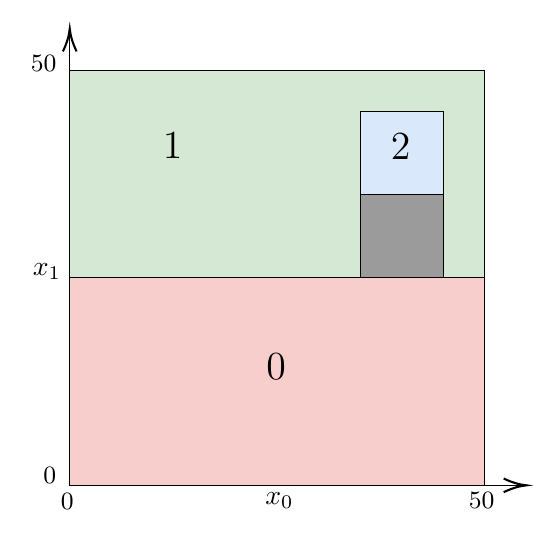
\begin{tikzpicture}[x=0.75pt,y=0.75pt,yscale=-1,xscale=1]
%uncomment if require: \path (0,300); %set diagram left start at 0, and has height of 300

%Shape: Rectangle [id:dp12943827359599314] 
\draw  [fill={rgb, 255:red, 213; green, 232; blue, 212 }  ,fill opacity=1 ] (250,50) -- (450,50) -- (450,150) -- (250,150) -- cycle ;
%Straight Lines [id:da8416607833401318] 
\draw    (250,250) -- (250,32) ;
\draw [shift={(250,30)}, rotate = 90] [color={rgb, 255:red, 0; green, 0; blue, 0 }  ][line width=0.75]    (10.93,-3.29) .. controls (6.95,-1.4) and (3.31,-0.3) .. (0,0) .. controls (3.31,0.3) and (6.95,1.4) .. (10.93,3.29)   ;
%Straight Lines [id:da5577600596159713] 
\draw    (250,250) -- (468,250) ;
\draw [shift={(470,250)}, rotate = 180] [color={rgb, 255:red, 0; green, 0; blue, 0 }  ][line width=0.75]    (10.93,-3.29) .. controls (6.95,-1.4) and (3.31,-0.3) .. (0,0) .. controls (3.31,0.3) and (6.95,1.4) .. (10.93,3.29)   ;
%Straight Lines [id:da17568384394881242] 
\draw    (250,150) -- (450,150) ;
%Shape: Rectangle [id:dp3705541448905584] 
\draw  [fill={rgb, 255:red, 248; green, 206; blue, 204 }  ,fill opacity=1 ] (250,150) -- (450,150) -- (450,250) -- (250,250) -- cycle ;
%Shape: Rectangle [id:dp5334639009219723] 
\draw  [fill={rgb, 255:red, 218; green, 232; blue, 252 }  ,fill opacity=1 ] (390,70) -- (430,70) -- (430,110) -- (390,110) -- cycle ;
%Shape: Rectangle [id:dp05533155300504711] 
\draw  [fill={rgb, 255:red, 155; green, 155; blue, 155 }  ,fill opacity=1 ] (390,110) -- (430,110) -- (430,150) -- (390,150) -- cycle ;

% Text Node
\draw (343.5,185.33) node [anchor=north west][inner sep=0.75pt]  [font=\Large]  {$0$};
% Text Node
\draw (293.6,79) node [anchor=north west][inner sep=0.75pt]  [font=\Large]  {$1$};
% Text Node
\draw (403.5,79.33) node [anchor=north west][inner sep=0.75pt]  [font=\Large]  {$2$};
% Text Node
\draw (343,252) node [anchor=north west][inner sep=0.75pt]    {$x_{0}$};
% Text Node
\draw (231,142) node [anchor=north west][inner sep=0.75pt]    {$x_{1}$};
% Text Node
\draw (244.5,252.67) node [anchor=north west][inner sep=0.75pt]  [font=\small]  {$0$};
% Text Node
\draw (236,240.33) node [anchor=north west][inner sep=0.75pt]  [font=\small]  {$0$};
% Text Node
\draw (230,41.67) node [anchor=north west][inner sep=0.75pt]  [font=\small]  {$50$};
% Text Node
\draw (441,252) node [anchor=north west][inner sep=0.75pt]  [font=\small]  {$50$};


\end{tikzpicture}

    \caption{Decision rule for the \dataset{CakeOnSea} dataset.}
    \label{fig:cake_on_sea}
\end{figure}

\subsection{\dataset{ForestCover}}

This dataset is taken from the UCI Machine Learning repository \cite{duaUCI2019} and can be found at this URL: \url{https://archive.ics.uci.edu/ml/datasets/Covertype}. 
It contains data on about 580000 trees such as their elevation, their horizontal distance to the nearest surface water features and the type of soil they are in, as well as their species (among seven tree species). There is a total of 13 recorded variables, including the tree species. Of the 12 variables used for prediction, two are categorical, and encoded as one-hot columns.
Because our method does not yet apply to categorical features, we remove the one-hot columns.

\subsection{\dataset{WineQuality}}

WineQuality: Around 6k rows. Response is quality from 0 to 10, but in fact there are no rows with quality 0, 1, 2 or 10, and 43\% of the rows have a rating of 6.
Hence we make the following mapping: class 0 corresponds to a quality rating of 5 or lower, class 1 to a rating of 6, and class 2 to a rating of 7 or higher.
With this mapping, around 33\% of data are in class 0, 43\% in class 1 and 18\% in class 2.

\end{document}